\section{Aufgabenstellung}
\label{sec:aufgabenstellung}

Bei dieser Bachelorarbeit werden die Flügelprofile des Ultraleichtdoppeldeckers FK12 Comet der Firma FK-Lightplanes untersucht. Die FK12 Comet ist weltweit der einzige in Serie hergestellte Ultraleichtdoppeldecker. Seit 2012 wird die FK12 Comet in der modifizierten Variante S2 hergestellt.  
Ultraleichtflugzeuge müssen in der Lage sein, mit der Geschwindigkeit von \SI{65}{km/h} (\SI{18.055}{m/s}) ohne Strömungsabriss fliegen zu können, woraus sich das zugelassene Abflug- und Landegewicht ergibt. Das maximal zugelassene Abflug- und Landegewicht für  das Flugzeug FK12 Comet S2 beträgt \SI{472.5}{\kilogram} und für das Flugzeug FK12 Comet S1 \SI{450}{\kilogram}.

Das Ziel der Bachelorarbeit ist, mit Hilfe von Strömungssimulationen herauszufinden, wie Vortexgeneratoren auf dem Flugzeugflügel S1 zu positionieren sind, damit bei der Geschwindigkeit von \SI{65}{km/h} ein höherer Auftrieb entsteht. Für das Ziel einer optimalen Aufrüstung des Flügelprofils S1 mit Vortexgeneratoren wird eine Parameterstudie durchgeführt, um herauszufinden, an welcher Position die Vortexgeneratoren platziert und welche Dimension die Vortexgeneratoren haben müssen. Mit dem höheren Auftrieb soll erreicht werden, dass das Flugzeug FK12 Comet S1 mit mehr Abflug- und Landegewicht zugelassen werden kann. Um die Wirkung der Vortexgeneratoren und den Übergang von laminarer zu turbulenter Strömung kennenzulernen, werden Simulationen mit Experimenten der technischen Universität von Dänemark \cite{Backus67} verglichen.
Zusätzlich soll der Unterschied zwischen den Landeklappenarten des Flugzeuges FK12 Comet S1 und S2 auf verschiedene Flugeigenschaften in der zweidimensionalen Simulation untersucht und verglichen werden. Aus dem Vergleich soll ersichtlich werden, welchen Einfluss die Modifizierung der Landeklappe auf den Auftrieb hat. Zusätzlich zum Vergleich der Landeklappen werden die Ergebnisse der zweidimensionalen Simulation mit den Messergebnissen der Flügelprofile aus dem Windkanal der Universität Stuttgart \cite{Bay00} verglichen. 
\newpage

\section{Motivation}
\label{sec:motivation}
In dieser Bachelorarbeit werden die Auswirkungen von Vortexgeneratoren auf dem Flugzeugflügel am Beispiel des Flugzeuges FK12 Comet S1 untersucht. Dabei soll das Flugzeug FK12 Comet S1 mit Vortexgeneratoren aufgerüstet werden, damit ein besserer Auftrieb entsteht und somit mit mehr Gewicht beladen werden darf. Zusätzlich wird die unterschiedliche Landeklappenart der Flugzeuge FK12 Comet S1 und S2 auf die verschiedenen Flugeigenschaften getestet. Beim Flügel mit einem Spalt zwischen Landeklappe und Flügelprofil wird in der folgenden Bachelorarbeit vom Flügelprofil S2 gesprochen. Beim Flügelprofil S1 handelt es sich um den Flügel, bei dem die Landeklappen in das Flügelprofil integriert sind.  In Folge wird genauer auf das Flugzeug eingegangen, auf das Wirkungsprinzip der Vortexgeneratoren sowie auf die Flügelprofile S1 und S2.


\paragraph{Flugzeug}
\label{subsec:flugzeug}
$\;$\\
Folgende Beschreibung trifft laut der Firma FK-Lightplanes \cite{Backus67} auf das Flugzeug zu: \guillemotleft{}Die FK12 COMET S2 ist der einzige ultraleichte, in Serie produzierte, Doppeldecker weltweit; handgefertigt für den ultimativen Flugspass. Sie ist ein sehr agiles, dabei aber gutmütiges Flugzeug für den sportlichen Piloten. Sie ist die konsequente Weiterentwicklung der erfolgreichen FK12 Comet S1, die bereits in 100 Exemplaren weltweit fliegt.

Die FK12 COMET S2 ist unvergleichlich, nicht nur in Ihrem sportlichen Design, sie ist zudem der schnellste Doppeldecker weltweit, im Verhältnis zu Ihrer Leistung von 100 PS. Die Tragflächen lassen sich von einer Person in wenigen Minuten anklappen, so dass sie überall Platz findet. 

Das moderne Querruder/Flaperon System ermöglicht der FK12 Comet S2 ein sehr agiles Flugverhalten, mit hoher Rollrate, bei gleichzeitig sehr guten Langsamflugeigenschaften. So kann die FK12 Comet S2 von jedem Piloten mit etwas Erfahrung sicher geflogen werden.\guillemotright{}\\
In Tabelle \ref{tab:flugzeugdaten_fk_12_s2} sind die technischen Spezifikationen des Flugzeuges FK12 Comet S2 aufgelistet. In Abbildung \ref{fig:foto_fk12_comet} ist ein Flugzeug FK12 Comet zu sehen.


\begin{table} [htb!]
\centering
\renewcommand{\arraystretch}{1.25}
    \begin{tabular}{|l|l|}
    \hline
    \textbf{Kenngrösse}    & \textbf{Daten} \\ \hline
    Sitze                                                                    & 2            \\ \hline
   Länge                                                                & 5.955 m                \\ \hline
       Höhe                                                                 & 2 m          \\ \hline
        Spannweite                                                           & 6.36                \\ \hline
        Flügelfläche                                                         & 13.4 m$^2$          \\ \hline
        Leergewicht                                                          & ca. 290 kg      \\ \hline
   max. Startgewicht                                                    & 540 kg                  \\ \hline
   \begin{tabular}[c]{@{}l@{}}max. Startgewicht\\ in CH/DE\end{tabular} & 472.5 kg           \\ \hline
   Höchstgeschwindigkeit                                                & 220 km/h          \\ \hline
  
    \end{tabular}
    \caption{Flugzeugdaten vom Flugzeug FK12 Comet S2 \cite{Bay00}}
        \label{tab:flugzeugdaten_fk_12_s2}
\end{table}


	\begin{figure}[htb!]
	\begin{center}
	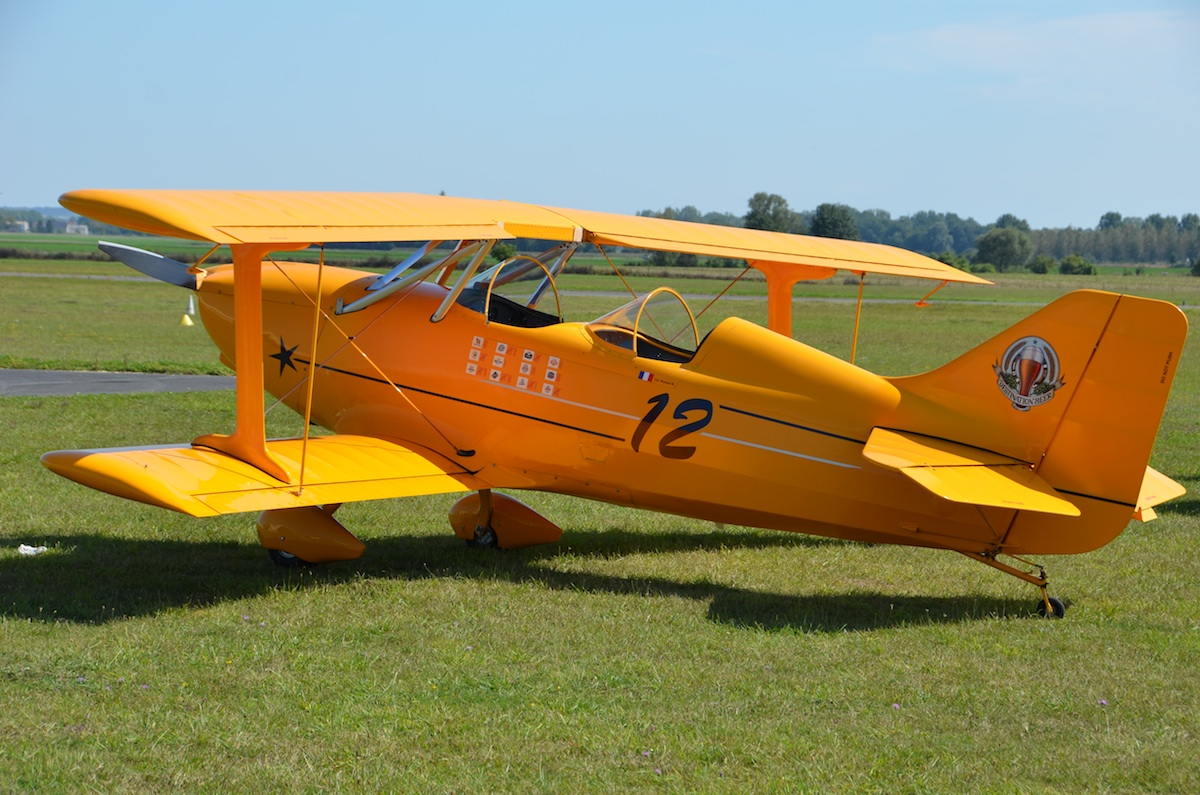
\includegraphics[width=0.48\textwidth]{fk12comet_kompl}
	\caption{Flugzeug FK12 Comet S1 \cite{Bay00}}
	\label{fig:foto_fk12_comet}
	\end{center}
	\end{figure}


... und so weiter ...
